%!TEX TS-program = xelatex
%!TEX encoding = UTF-8 Unicode

\documentclass[12pt]{extarticle}
% extarticle is like article but can handle 8pt, 9pt, 10pt, 11pt, 12pt, 14pt, 17pt, and 20pt text

\def \ititle {Origins of Mind}
 
\def \isubtitle {Lecture 06}
 
\def \iauthor {Stephen A. Butterfill}
\def \iemail{s.butterfill@warwick.ac.uk}
\date{}

%for strikethrough
\usepackage[normalem]{ulem}

\input{$HOME/Documents/submissions/preamble_steve_handout}

%\bibpunct{}{}{,}{s}{}{,}  %use superscript TICS style bib
%remove hanging indent for TICS style bib
%TODO doesnt work
\setlength{\bibhang}{0em}
%\setlength{\bibsep}{0.5em}


%itemize bullet should be dash
\renewcommand{\labelitemi}{$-$}

\begin{document}

\begin{multicols}{3}

\setlength\footnotesep{1em}


\bibliographystyle{newapa} %apalike

%\maketitle
%\tableofcontents




%--------------- 
%--- start paste
\def \ititle {Origins of Mind}
 
\def \isubtitle {Lecture 06}
 
 
 
\
 
 
 
\begin{center}
 
{\Large
 
\textbf{\ititle}: \isubtitle
 
}
 
 
 
\iemail %
 
\end{center}
 
‘there are many separable systems of mental representations ... and thus many different kinds of knowledge. ... the task ... is to contribute to the enterprise of finding the distinct systems of mental representation and to understand their development and integration’
\citep[p.\ 1522]{Hood:2000bf}.
 
 
 
\section{Core Knowledge: First Pass}
 
For someone to have \textit{core knowledge of a particular principle or fact} is for her to have a core system where 
either the core system includes a representation of that principle or else the principle plays a special role in describing the core system.
 
\subsection{Two-part definition}
 
‘Just as humans are endowed with multiple, specialized perceptual systems, so we are endowed with multiple systems for representing and reasoning about entities of different kinds.’
\citep[p.\ 517]{Carey:1996hl}
 
‘core systems are 
largely innate 
encapsulated 
unchanging 
arising from phylogenetically old systems 
built upon the output of innate perceptual analyzers’ 
\citep[p.\ 520]{Carey:1996hl}.
 
\textit{Note} There are other, slightly different statements \citep[e.g.][]{carey:2009_origin}.
 
 
 
\section{Core Knowledge: Objections}
 
‘We hypothesize that uniquely human cognitive achievements build on systems that humans 
share with other animals: core systems that evolved before the emergence of our species. 
The internal functioning of these systems depends on principles and processes that are 
distinctly non-intuitive.  Nevertheless, human intuitions about space, number, morality 
and other abstract concepts emerge from the use of symbols, especially language, to 
combine productively the representations that core systems deliver’
\citep[pp.\ 2784-5]{spelke:2012_core}.
\citep[p.\ 517]{Carey:1996hl}
 
\subsection{Objection}
 
‘there is a paucity of … data to suggest that they are the only or the best way of carving up the processing,
 
‘and it seems doubtful that the often long lists of correlated attributes should come as a package’
\citep[p.\ 759]{adolphs_conceptual_2010}
 
‘we wonder whether the dichotomous characteristics used to define the two-system models are … perfectly correlated …
[and] whether a hybrid system that combines characteristics from both systems could not be … viable’
\citep[p.\ 537]{keren_two_2009}
 
‘the process architecture of social cognition is still very much in need of a detailed theory’
\citep[p.\ 759]{adolphs_conceptual_2010}
 
 
 
\section{Core Knowledge and Modularity}
 
‘In Fodor’s (1983) terms, visual tracking and preferential looking each may depend on modular mechanisms.’
\citep[p.\ 137]{spelke:1995_spatiotemporal}
 
\subsection{Modularity}
 
Fodor’s three claims about modules:
 
\begin{enumerate}
 
\item they are ‘the psychological systems whose operations present the world to thought’;
 
\item they ‘constitute a natural kind’; and
 
\item there is ‘a cluster of properties that they have in common’ \citep[p.\ 101]{Fodor:1983dg}.
 
\end{enumerate}
 
These properties include:
 
\begin{itemize}
 
\item domain specificity (modules deal with ‘eccentric’ bodies of knowledge)
 
\item limited accessibility (representations in modules are not usually inferentially integrated with knowledge)
 
\item information encapsulation (modules are unaffected by general knowledge or representations in other modules)
 
\item innateness (roughly, the information and operations of a module not straightforwardly consequences of learning; but see \citet{Samuels:2004ho}).
 
\end{itemize}
 
 
 
\section{Syntax / Innateness}
 
Is the syntactic structure of ‘the red ball’ (a) flat or (b) hierachical?
 
\begin{center}
 
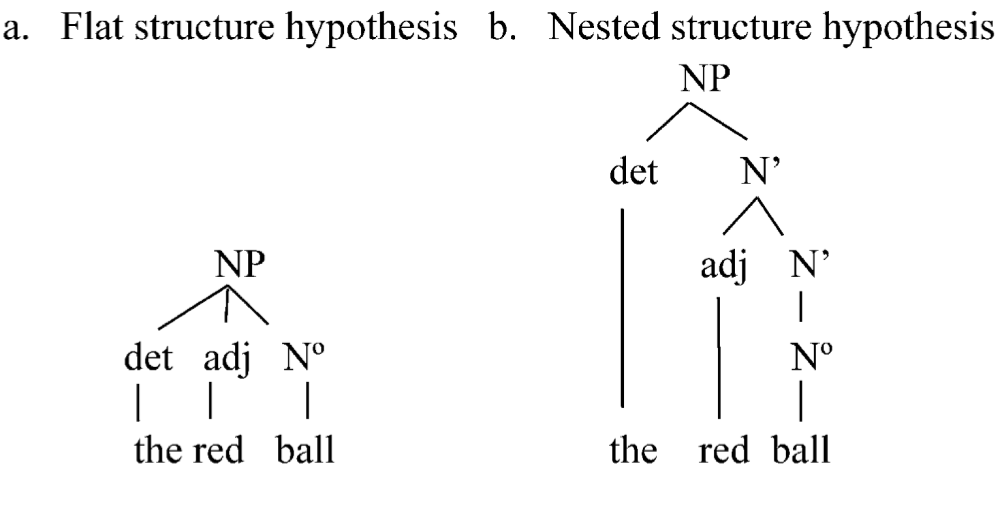
\includegraphics[scale=0.25]{../www.slides/src/raw/img/lidz_2003_fig0.neg.png}
 
\end{center}
 
\begin{center} from \citealp{lidz:2003_what} \end{center}
 
\begin{enumerate}
\item ‘red ball’ is a constituent on (b) but not on (a)
\item anaphoric pronouns can only refer to constituents
\item In the sentence ‘I’ll play with this red ball and you can play with that one.’, the word ‘one’ is an anaphoric prononun that refers to ‘red ball’ (not just ball).
\citep{lidz:2003_what,lidz:2004_reaffirming}.
 
\end{enumerate}
 
‘The assumption in the preferential looking task is that infants prefer to look at an image that matches the linguistic stimulus, if one is available’ \citep{lidz:2003_what}.
 
\subsection{Poverty of stimulus arguments}
 
How do poverty of stimulus arguments work? See \citet{pullum:2002_empirical}.
 
\begin{enumerate}
 
\item
 
Human infants acquire X. 
 
\item
 
To acquire X by data-driven learning you'd need this  Crucial Evidence. 
 
\item
 
But infants lack this Crucial Evidence for X.
 
\item
 
So human infants do not acquire X by data-driven learning.
 
\item
 
But all acquisition is either data-driven or innately-primed learning.
 
\item
 
So human infants acquire X by innately-primed learning .
 
\end{enumerate}
 
‘the APS [argument from the poverty of stimulus] still awaits even a single good supporting example’
\citep[p.\ 47]{pullum:2002_empirical}
     
 
 
%--- end paste
%--------------- 
 
\footnotesize 
\bibliography{$HOME/endnote/phd_biblio}

\end{multicols}

\end{document}